\section*{33. Магнитное поле в среде. Молекулярные токи. Вектор намагниченности,
его связь с молекулярными токами.}

\subsection*{Молекулярные токи и Вектор намагниченности,
его связь с молекулярными токами}

\begin{minipage}[c]{0.25\textwidth} % Левая часть: изображение
    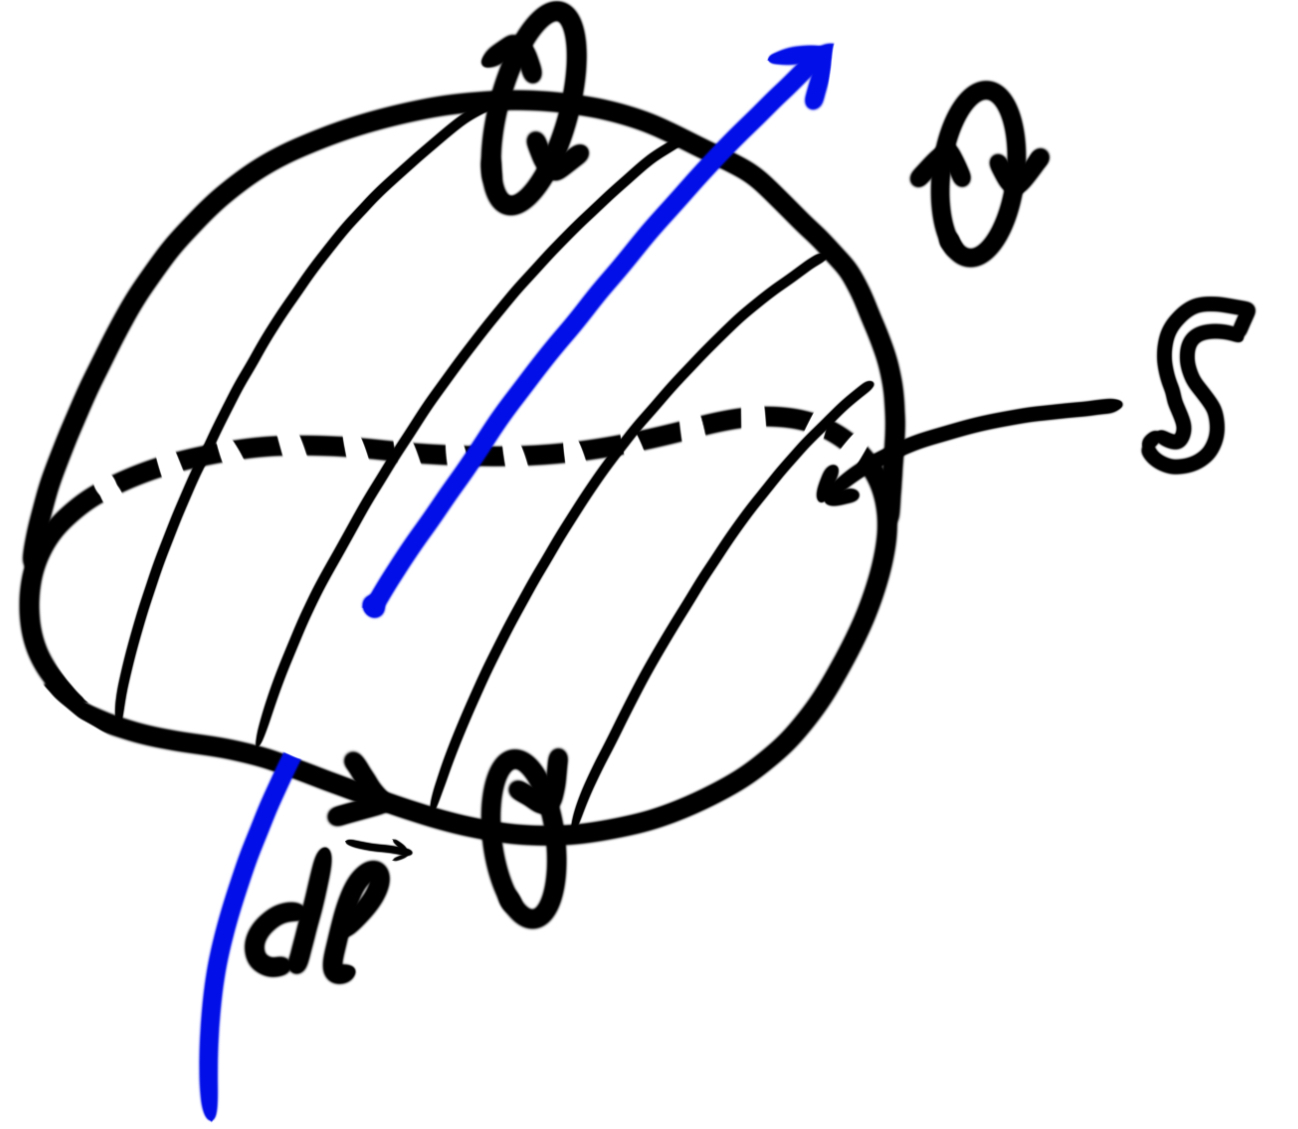
\includegraphics[width=\textwidth]{im/72.png} % Ваше изображение
\end{minipage}%
\hfill
\begin{minipage}[c]{0.7\textwidth} % Правая часть: текст
    \begin{gather*}
        I_{\text{м}}=\underset{S}{\iint} <\vec{j}_{\text{м}}>d\vec{S}=\iint \vec{j}_{\text{м}}d\vec{S}=c\oint \vec{M}d\vec{l}= \\
        =c\underset{S}{\iint}\mathrm{rot}\vec{M}dS \Rightarrow <\vec{j}_{\text{м}}>\overset{df}{=}c\cdot \mathrm{rot}\vec{M} \\
        M\text{- ветктор намагниченности, вне тела } M=0
    \end{gather*}
\end{minipage}

\subsection*{Магнитное поле в среде}

\[
\begin{aligned}
    \begin{cases}
        \mathrm{div}\vec{H}=0  \\ 
        \mathrm{rot}\vec{H}=\frac{4\pi}{c}(\vec{j}+\vec{j}_{\text{м}})
    \end{cases}
    \overset{\text{уср}}{\rightarrow}
    \begin{cases}
        \quad \mathrm{div}<\vec{H}>=0 \\
        \mathrm{rot}<\vec{H}= \frac{4\pi}{c}(\vec{j}+<\vec{j}_{\text{м}}>)
    \end{cases}
    \rightarrow
\end{aligned}
\]

\[
\begin{aligned}
    \overset{<\vec{H}>=:\vec{B}}{\rightarrow}
    \begin{cases}
        \mathrm{div}\vec{B}=0 \\
        \mathrm{rot}\vec{B}= \frac{4\pi}{c}(\vec{j}+<\vec{j}_{\text{м}}>)
    \end{cases}
    \overset{<\vec{j}_{\text{м}}>=c\cdot \mathrm{rot}\vec{M}}{\rightarrow}
    \begin{cases}
        \mathrm{div}\vec{B}=0 \\
        \mathrm{rot}(\vec{B}-4\pi\vec{M})= \frac{4\pi}{c}\vec{j}
    \end{cases}
    \rightarrow 
\end{aligned}
\]

\[
\begin{aligned}
    \overset{\vec{B}-4\pi\vec{M}=:\vec{H}}{\rightarrow}
    \boxed{\begin{cases}
        \mathrm{div}\vec{B}=0 \\
        \mathrm{rot}\vec{H}= \frac{4\pi}{c}\vec{j}
    \end{cases}
    }
\end{aligned}
\]

Дополнительная информация:

\[
\vec{M}=\vec{H}\chi, \chi \text{-намагничиваемость} 
\]

\[
\vec{B}=\mu \vec{H}, \mu \text{-магнитная проводимость}
\]

\[
\mu=1+4\pi\chi
\]